\documentclass[a4paper,12pt]{report}
\usepackage[a4paper,inner = 0.5cm, outer = 0.5cm, top = 2cm, bottom = 2cm]{geometry}

\usepackage[english,romanian]{babel}
\usepackage{blindtext}
\usepackage{fancyhdr}
\usepackage{wrapfig}
\usepackage{graphicx}
\usepackage{amsmath}
\usepackage{caption}
\usepackage{dirtytalk}
\usepackage{url}
\usepackage{listings}

\renewenvironment{abstract}[1]
  {\bigskip\selectlanguage{#1}%
   \begin{center}\bfseries\abstractname\end{center}}
  {\par\bigskip}

\newcommand{\source}[1]{\caption*{Sursă: {#1}} }

\fancyhf{}
\renewcommand{\headrulewidth}{2pt}
\renewcommand{\footrulewidth}{1pt}
\fancyhead[LE]{\leftmark}
\fancyhead[RO]{\rightmark}
\linespread{1.25}
\hyphenpenalty=50000
\begin{document}
\begin{titlepage}
    \begin{center}
        \begin{figure}[htbp]
            \centering
            \begin{minipage}{0.2\textwidth}
              
\includegraphics[width=\linewidth]{images/poza_stanga.png}
            \end{minipage}\
            \begin{minipage}{0.5\textwidth}
                \begin{large}
                    \textbf{UNIVERSITATEA DIN BUCUREȘTI}\\
                    \\
                    \begin{center}
                    \textbf{FACULTATEA\\
                                DE\\
                    MATEMATICĂ ȘI INFORMATICĂ}
								\end{center}
                \end{large}
            \end{minipage}
            \begin{minipage}{0.2\textwidth}
              
\includegraphics[width=\linewidth]{images/poza_dreapta.png}
            \end{minipage}
        \end{figure}
        
        \vspace*{1cm}
        
        \begin{large}
            \textbf{SPECIALIZAREA INFORMATICĂ}
        \end{large}

        \vspace{2.5cm}
        \begin{LARGE}
            \textbf{LUCRARE DE DISERTAŢIE}\\
            \vspace*{0.5cm}
            \textbf{EXECUŢIA WORKFLOW-URILOR DURABILE ÎN CLOUD}
        \end{LARGE}
            
        \vspace{2.5cm}
        \begin{large}
            \textbf{Absolvent}\\
            \vspace*{0.25cm}
            \textbf{Moldovan George-Alexandru}
        \end{large}
        
        \vspace{2cm}
        \begin{large}
            \textbf{Coordonator științific}\\
            \vspace*{0.25cm}
            \textbf{Prof. dr. Letiţia Marin}
        \end{large}
        
        \vspace{2.5cm}
        \begin{large}
            \textbf{București, septembrie 2022}
        \end{large}
    \end{center}
\end{titlepage}
\newgeometry{a4paper,inner = 1.7cm, outer = 2.7cm, top = 2cm, bottom = 2cm, bindingoffset = 1.2cm}
\begin{abstract}{romanian}
\par Considerând trend-ul ascendent al arhitecturii orientate spre microservicii si migrarea de la vechiul mod de dezvoltare monolit, aceasta lucrare de disertaţie işi propune analiza soluţiilor prezente in piaţa în ceea ce priveşte managementul unei arhitecturi pe microservicii în cloud, şi analiza unor contribuţii personale aduse unui framework open-source de gestionare a workflow-urilor în cloud. Sistemele informatice preiau din complexitatea operaţiilor de zi cu zi, astfel că arborii de decizie trebuie interpretaţi şi gestionaţi în mod corect pentru a realiza un sistem care sa indeplinească cerinţele de piaţă curente. Pentru o lunga perioadă de timp, problema gestionării tranzacţiilor distribuite si management-ul workflow-urilor a fost inexistentă, deoarece într-un sistem monolit, caracteristicile tranzacţionale ale bazelor de date ce susţineau astfel de sisteme erau indeajuns pentru a avea toate garanţiile necesare astfel încât sistemul sa fie mereu lăsat într-o stare consistentă. Microserviciile şi arhitecturile distribuite in general, deşi vin cu o serie lunga de avantaje, poate cel mai greu de gestionat lucru este management-ul stării unei acţiuni, atunci cand aceasta se întinde pe mai multe microservicii, şi pe o durată lungă de timp. 
\end{abstract}
\begin{abstract}{english}\par Considering the upward trend of microservices-oriented architecture and the migration from the old monolithic development mode, this dissertation aims to analyze the solutions present in the market in terms of managing a microservices architecture in the cloud, and the analysis of personal contributions to a open-source framework for managing cloud workflows. Information systems take over the complexity of day-to-day operations, so decision trees must be interpreted and managed correctly to achieve a system that meets current market requirements. For a long time, the problem of distributed transaction management and workflow management was non-existent, because in a monolithic system, the transactional characteristics of the databases that supported such systems were sufficient to have all the necessary guarantees so that the system should always be left in a consistent state. Distributed microservices and architectures in general, although they come with a long list of advantages, perhaps the most difficult thing to manage is the management of the state of an action, when it extends over several microservices, and over a long period of time.
\end{abstract}
\tableofcontents
\pagenumbering{arabic}
\setcounter{page}{2}
\chapter{Introducere}
\section{Motivatie}
\quad Unul din principiile de baza ale programării este reutilizarea. Motivaţia din spatele acestei lucrări o reprezintă dorinţa de o contribui la un framework care rezolvă o problemă generică, cu care se confruntă toţi dezvoltatorii care trebuie sa gestioneze tranzacţii distribuite. Analiza diferitelor metode pentru rezolvarea problemei de gestiune a workflow-urilor în cloud, în special într-o arhitectură ce se bazează pe funcţii în cloud a fost o prioritate pentru mine în ultimii ani. 
\par
Serverless, sau Functions-as-a-Service (FaaS), este o paradigmă din ce în ce mai populară pentru dezvoltarea de aplicații, deoarece oferă scalare infintă implicită și facturare bazată pe consum. Cu toate acestea, garanţiile slable de execuţie și suportul nativ pentru stocare a stării a FaaS creează provocări serioase atunci când se dezvoltă aplicații care necesită stare persistentă, garanţii de execuţie sau sincronizare. Acest lucru a motivat o nouă generație de soluţii serverless care oferă abstractizări ce stochează starea aplicaţiei. De exemplu, noua soluţie Azure Durable Functions (DF), o extindere peste deja existenta Azure Functions. Modelul îmbunătățește FaaS cu actori, fluxuri de lucru și secțiuni critice.
\par
În acest context în care dezvoltatorii incearcă sa dezvolte aplicaţii ce gestiunează workflow-uri  de lungă durată, cu toţii rezolvă aceeaşi problemă şi anume lipsa separării intre nivelul de execuţie si nivelul de stocare a soluţiilor existente FaaS. Cu toţii rezolvă o problemă generică, de salvare a stării în anumite puncte ale execuţiei, pentru a putea relua workflow-ul în eventualitatea în care agentul pe care rulează aplicaţie pică inainte de finalizarea workflow-ului. Acest lucru era foarte greu de realizat in arhitecturi serverless deoarece toate soluţiile existente până la apariţia Azure Durable Functions, suportau doar execuţii stateless în mod standard. Deci până la apariţia soluţiilor ce oferă garanţii de execuţie puternice in lumea Serverless, această tehnologie nu era o opţiune populară pentru dezvoltarea aplicaţiilor ce aveau nevoie de gestionare a stării şi era limitată la execuţia unor parţi mici ale aplicaţiilor pentru care starile intermediare nu erau importante. 
\section{Context}
\quad Serverless diferă de conceptele tradiționale de cloud computing în sensul că infrastructura și platformele în care serviciile rulează sunt ascunse clienților. În această abordare, clienții sunt preocupați doar de funcționalitatea dorită a aplicației lor, iar restul este delegată furnizorului de servicii. \par

Scopul serviciilor Serverless este triplu : 
\begin{itemize}
\item Scuteşte dezvoltatorii de servicii cloud de la interacţiunea cu infrastructura sau diferite platforme
\item Converteste modelul de facturare din cel clasic la cel bazat pe consum
\item Scalarea automată a serviciului în funcție de cererea clienților.
\end{itemize}
\par

\begin{wrapfigure}{r}{0.45\textwidth}
	  \begin{center}
        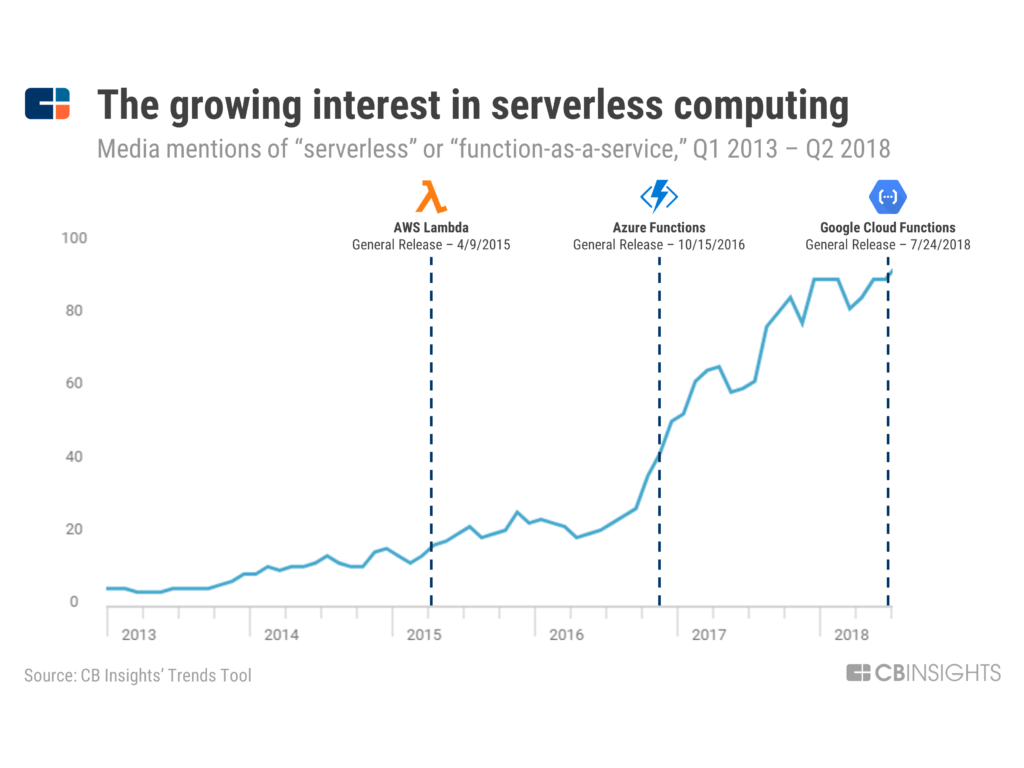
\includegraphics[width=0.4\textwidth]{images/grafic_serverless_computing}
       \caption{Statistică ce evidenţiază importanţa domeniului cloud computing în ultimii ani}
			\label{fig:cloud_computing_graph}
       \source {https://www.cbinsights.com}
    \end{center}
\end{wrapfigure}
Ca rezultat, într-o aplicație cu adevărat Serverless, infrastructura de execuție este ascunsă clientului, iar clientul plătește doar pentru resursele pe care le utilizează efectiv. Serviciul este conceput astfel încât să poată gestiona rapid creșterile de consum prin scalare automată. Entitățile de bază în calculul fără server sunt funcții. Clientul își înregistrează funcțiile în furnizorul de servicii. Apoi, acele funcții pot fi invocate fie de un eveniment, fie direct prin apelarea acestora la cererea utilizatorilor. Rezultatele execuției sunt trimise înapoi clientului. Invocarea funcțiilor este delegată unuia dintre nodurile de calcul disponibile în interiorul furnizorului de servicii. De obicei, aceste noduri sunt containere cloud, cum ar fi Docker [100] sau un mediu de rulare izolat [67].

\par
Deși conceptul de Serverless este relativ nou, acesta și-a deschis drumul în multe aplicații din lumea reală, de la instrumente de colaborare online la sisteme integrate (IoT), având o creştere în adopţie foarte rapidă, lucru vizibil şi în figura ~\ref{fig:cloud_computing_graph}. Această creştere este datorată în mare parte usurinţei proceselui de dezvoltare a aplicaţiilor Serverless şi beneficiile pe care le aduc din punct de vedere al scalării în mod automat, şi a gestionării complete a infrastructurii ce stă la baza aplicaţiilor. 
\par
Unul din lucrurile care poate duce adopţia tehnologiei serverless la un cu totul alt nivel, este tocmai capacitatea de a putea dezvolta aplicaţii intregi, ce se pot baza pe starea sistemului în cadrul execuţiei şi capacitatea de a gestiona long running workflows, o nevoie care este prezentă în mai toate aplicaţiile curente. 
\section{Alte analize ale problemelor curente a arhitecturii Serverless}
\quad Există mai multe provocări cu care se confruntă în prezent serviciile Serverless. Există unele sondaje și recenzii ale literaturii care discută aceste provocări \cite{baldini2017,rajkumar2017,paul2019,hassan2017,jonas2019}.
\par\emph{Baldini et al.} \cite{baldini2017} enumeră o serie de probleme cu care se confruntă arhitectura serverless, printre care costul, care reprezintă un avantaj pentru aceasta arhitectura doar dacă se execută metode care nu sunt bazate pe prelucrare input-output. Altfel, este mai eficient din punct de vedere al costurilor folosirea soluţiilor clasice în cloud cum ar fi maşini virtuale rezervata sau containere. O altă problemă semnalată este cea a cold-start-ului care poate face o aplicaţie bazata pe funcţii serverless sa pară înceată daca pentru fiecare apel este necesar un cold start, din cauză ca traficul nu este indeajuns de mult pentru a împiedica funcţia sa scaleze la 0. 
\par\emph{Rajkumar et al.} \cite{rajkumar2017} discută despre dificultăţile dezvoltării unei arhitecturi serverless din punct de vedere al limitărilor cu care vine această noua tehnologie si anume limitările de timp al executiei, de memorie al agentului si de management al stării. Acesta crede că este nevoie de o schimbare a mentalităţii de dezvoltare a aplicaţiilor pentru a benefecia la adevaratul său potenţial de tehnologiile Serverless, iar momentul în care aplicaţiile enterpise complete vor fi migrate sau dezvoltate complet pe o arhitectură Serverless este înca departe. Acesta vede această tehnologie ca pe o unealtă ajutătoare în dezvoltarea aplicaţiilor, dar pe viitor poate ajunge să fie nucleul aplicaţiilor.  
\par\emph{Castro et al.} \cite{paul2019} ridică problema dezvoltării de aplicaţii statefull folosind tehnologii Serverless in viitor, o temă ce in aceea perioadă era doar o idee, dar după cum urmează sa fie prezentat în aceasta lucrare, acum este o realitate. Alte probleme menţionate ar fi usurinţa cu care poate fi portată o aplicaţie legacy către o arhitectură Serverless, deoarece nu este de dorit sa se piardă toate acele ora valoroase care au fost deja investite în aplicaţiile existente. 
\par\emph{Hassan et al.} \cite{hassan2017} discuta despre problema limitării la un singur provider atunci cand vine vorba de arhitecturi serverless, deoarece codul pentru un anumit provider de exemplu AWS Lambda, nu e portabil către alt provider, de exemplu Microsoft Azure Functions. 
\par\emph{Jonas et al.} \cite{jonas2017} prezintă ineficienţele arhitecturii serverless atunci când vine vorba de procesarea operaţiilor care în mod normal ar beneficia de pe urma unui sistem cu mai multe nuclee, şi implicaţiile pe care aceasta limitare (2 nuclee per funcţie) o are atunci când vine vorba de paralelizarea acţiunilor pentru a îmbunăţăţii viteza. Impactul major în acest caz este creşterea semnificativă a datelor transmise pe reţea pentru a obţine acelasi grad de paralelism într-un sistem serverless versul unul clasic în cloud. 


\section{Conţinutul lucrării}
 Din punct de vedere al structurii, lucrarea va fi împărţită în 2 părţi :
\begin{itemize}
\item Partea teoretică în care va fi analizat Durable Task Framework şi cum funcţionează acesta
\item Partea practică ce va compara aceaşi aplicaţie, dezvoltată în 2 moduri (clasic şi folosind DTF)
\end{itemize}
\par În prima parte a lucrării va fi analizată tehnologia ce stă la baza soluţiilor de management a workflow-uri în cloud si anume, Durable Task Framework. Vom analiza modul în care este separat domeniul de execuţie de domeniul de stocare, care sunt interfeţele pe care trebuie sa le respecte un provider, care sunt constrângerile care trebuie respectate atunci se foloseste această tehnologie si bineînteles care sunt beneficiile si dezavantajele sale. 
\par În a 2a parte va fi analizat un exemplu clasic în literatura managementului de workflow-uri si anume cazul de rezervare multiplă în cazul unei călatorii. Această mini-aplicaţie a fost dezvoltată atât folosind metode clasice, cât şi folosind Durable Task Framework. Folosind aceste 2 abordari, vor fi analizate : 
\begin{itemize}
\item Capaciţăţile fiecărui sistem si nivelul de rezilienţă împotriva dezastrelor pe care îl pot demonstra
\item Diferenţele de dezvoltare între cele 2 abordări
\item Analiză teoretică a costurilor între cele 2 arhitecturi 
\item Performanţa celor 2 sisteme
\end{itemize}
\chapter{Analiza Tehnologiei Durable Task Framework si a providerilor disponibili}
\section{Analiză generală}
\quad Durable Task Framework (DTFx) este o bibliotecă care permite utilizatorilor să gestioneze workflow-uri persistente de lungă durată (denumite orchestrari) în C\# folosind sintagme clasica de codare async/await. DTF stă la baza soluţiilor Microsoft de gestionare a workflow-urilor durabile în cloud, şi folosind această tehnologie, a fost expusă prima soluţie serverless ce permite gestionarea stării : Azure Durable Functions. 
\par Din punct de vedere al arhitecturii framework-ului, acesta are 2 părti:
\begin{itemize} 
\item DTF Core ce conţine nivelul de abstractizare al gestionării, şi care implementează conceptele de bază ce permit programarea orchestrărilor folosind sintagme async await
\item DTF providers, care implementează interfeţele expuse de Core pentru a folosi diferite medii de stocare, în funcţie de nevoile dezvoltatorului. 
\end{itemize} 
\par La bază, framework-ul îşi propune să rezolve problema durabilităţii acţiunilor într-un sistem distribuit, în care este de aşteptat ca orice piesă a sistemului poate pica în orice moment. Arhitectura framework-ului e bazată pe evenimente, spre deosebire de alte framework-uri anterioare ce se bazau pe stocarea întregii stări a aplicaţiei la un moment dat. 
\par Nevoia de garanţii de execuţie a facut ca DTF să construiască un sistem ce permite construcţia unei structuri arborescente ce reprezintă o maşină de stări finite, în care, frunzele arborelui (Activităţile, în terminologia DTF) au garanţia că vor fi executate cel puţin odata. Această garanţie vine şi cu o constrângere : Din cauză că Activităţile nu sunt executate \textbf{exact o dată} este necesar ca toate acţiunile din cadrul unei Activităţi sa fie idempotente. 
\section{Folosirea evenimentelor în DTF}
\quad Modelul de arhitectură bazat pe evenimente este un model popular de arhitectură asincronă distribuită, utilizat pentru a produce aplicații foarte scalabile. De asemenea, este foarte adaptabil și poate fi utilizat pentru aplicații mici și, de asemenea, pentru cele mari și complexe. Arhitectura bazată pe evenimente este alcătuită din componente de procesare a evenimentelor extrem de decuplate, cu un singur scop, care primesc și procesează evenimentele în mod asincron.

Modelul de arhitectură bazat pe evenimente constă din două topologii principale, mediatorul și brokerul. Topologia mediatorului este folosită în mod obișnuit atunci când există nevoia de orchestrare a mai multor pași în cadrul unui eveniment printr-un mediator central, în timp ce topologia brokerului este utilizată atunci când doriți să înlănțuiți evenimente fără a utiliza un mediator central. Deoarece caracteristicile arhitecturii și strategiile de implementare diferă între aceste două topologii, este important ca ambele să fie cunoscute pentru a putea întelege motivaţie din spatele alegerii arhitecturii DTF. 

\par Gestionarea workflow-urilor prin mediator central cunoscută si drept \textbf{Orchestrare} în literatura de specialiate (\emph{Megargel et al.}\cite{megargel2021}), constă în prezenţa unei entităţi centrale ce comunică cu toate celelalte sisteme ce iau parte la un anume workflow pentru a garanta execuţia cu success a unei maşini de stări. Topologia mediatorului este utilă pentru evenimentele care au mai mulți pași și necesită un anumit nivel de orchestrare pentru a procesa evenimentul. Aşa cum vom vedea şi în partea practică a acestei lucrări, sunt nenumărate cazuri ce se reduc la gestionarea unei maşini de stări. Un astfel de exemplu este un lant de aprovizionare, în care, de la momentul achizitiei pana la momentul livrării sunt numeroase etape ce trebuiesc îndeplinite cu success pentru ca operaţiunea ca un întreg sa fie un success. Printre acest etape s-ar numara pregătirea coletului, predarea lui către firma de curierat, înregistrarea plăţii şi în final, livrarea propriu zisă. Un astfel de sistem poate benefie de un mediator central, care asigură gestiunea stării unui astfel de workflow. 
\par Gestionarea workflow-urilor printr-o topologie cu broker, cunoscută drept  \textbf{Coreografie}, constă în distribuirea gestiunii maşinii de stări între toti consumatorii evenimentelor, astfel fiecare poate lua o anumită decizie în funcţie de contextul în care se află atunci când procesează un eveniment. În această topologie, nu există un mediator central, iar fiecare participant în workflow are responsabilitatea deciderii următoarei acţiuni, în momentul procesării unui eveniment. Astfel, acest gen de arhitectură este potrivită pentru worfklow-uri minimale, făra maşini de stări complicate, care nu au nevoie de un loc centralizat pentru asigurarea consistenţei stării. Altfel, folosind această arhitectură în sisteme complexe, se poate ajunge foarte repede la haos, deoarece deciziile sunt împărtiţe peste tot, devenind imposibilă urmărirea firului logic al unei astfel de execuţii distribuite. 
\begin{figure}[h]
\begin{center}
        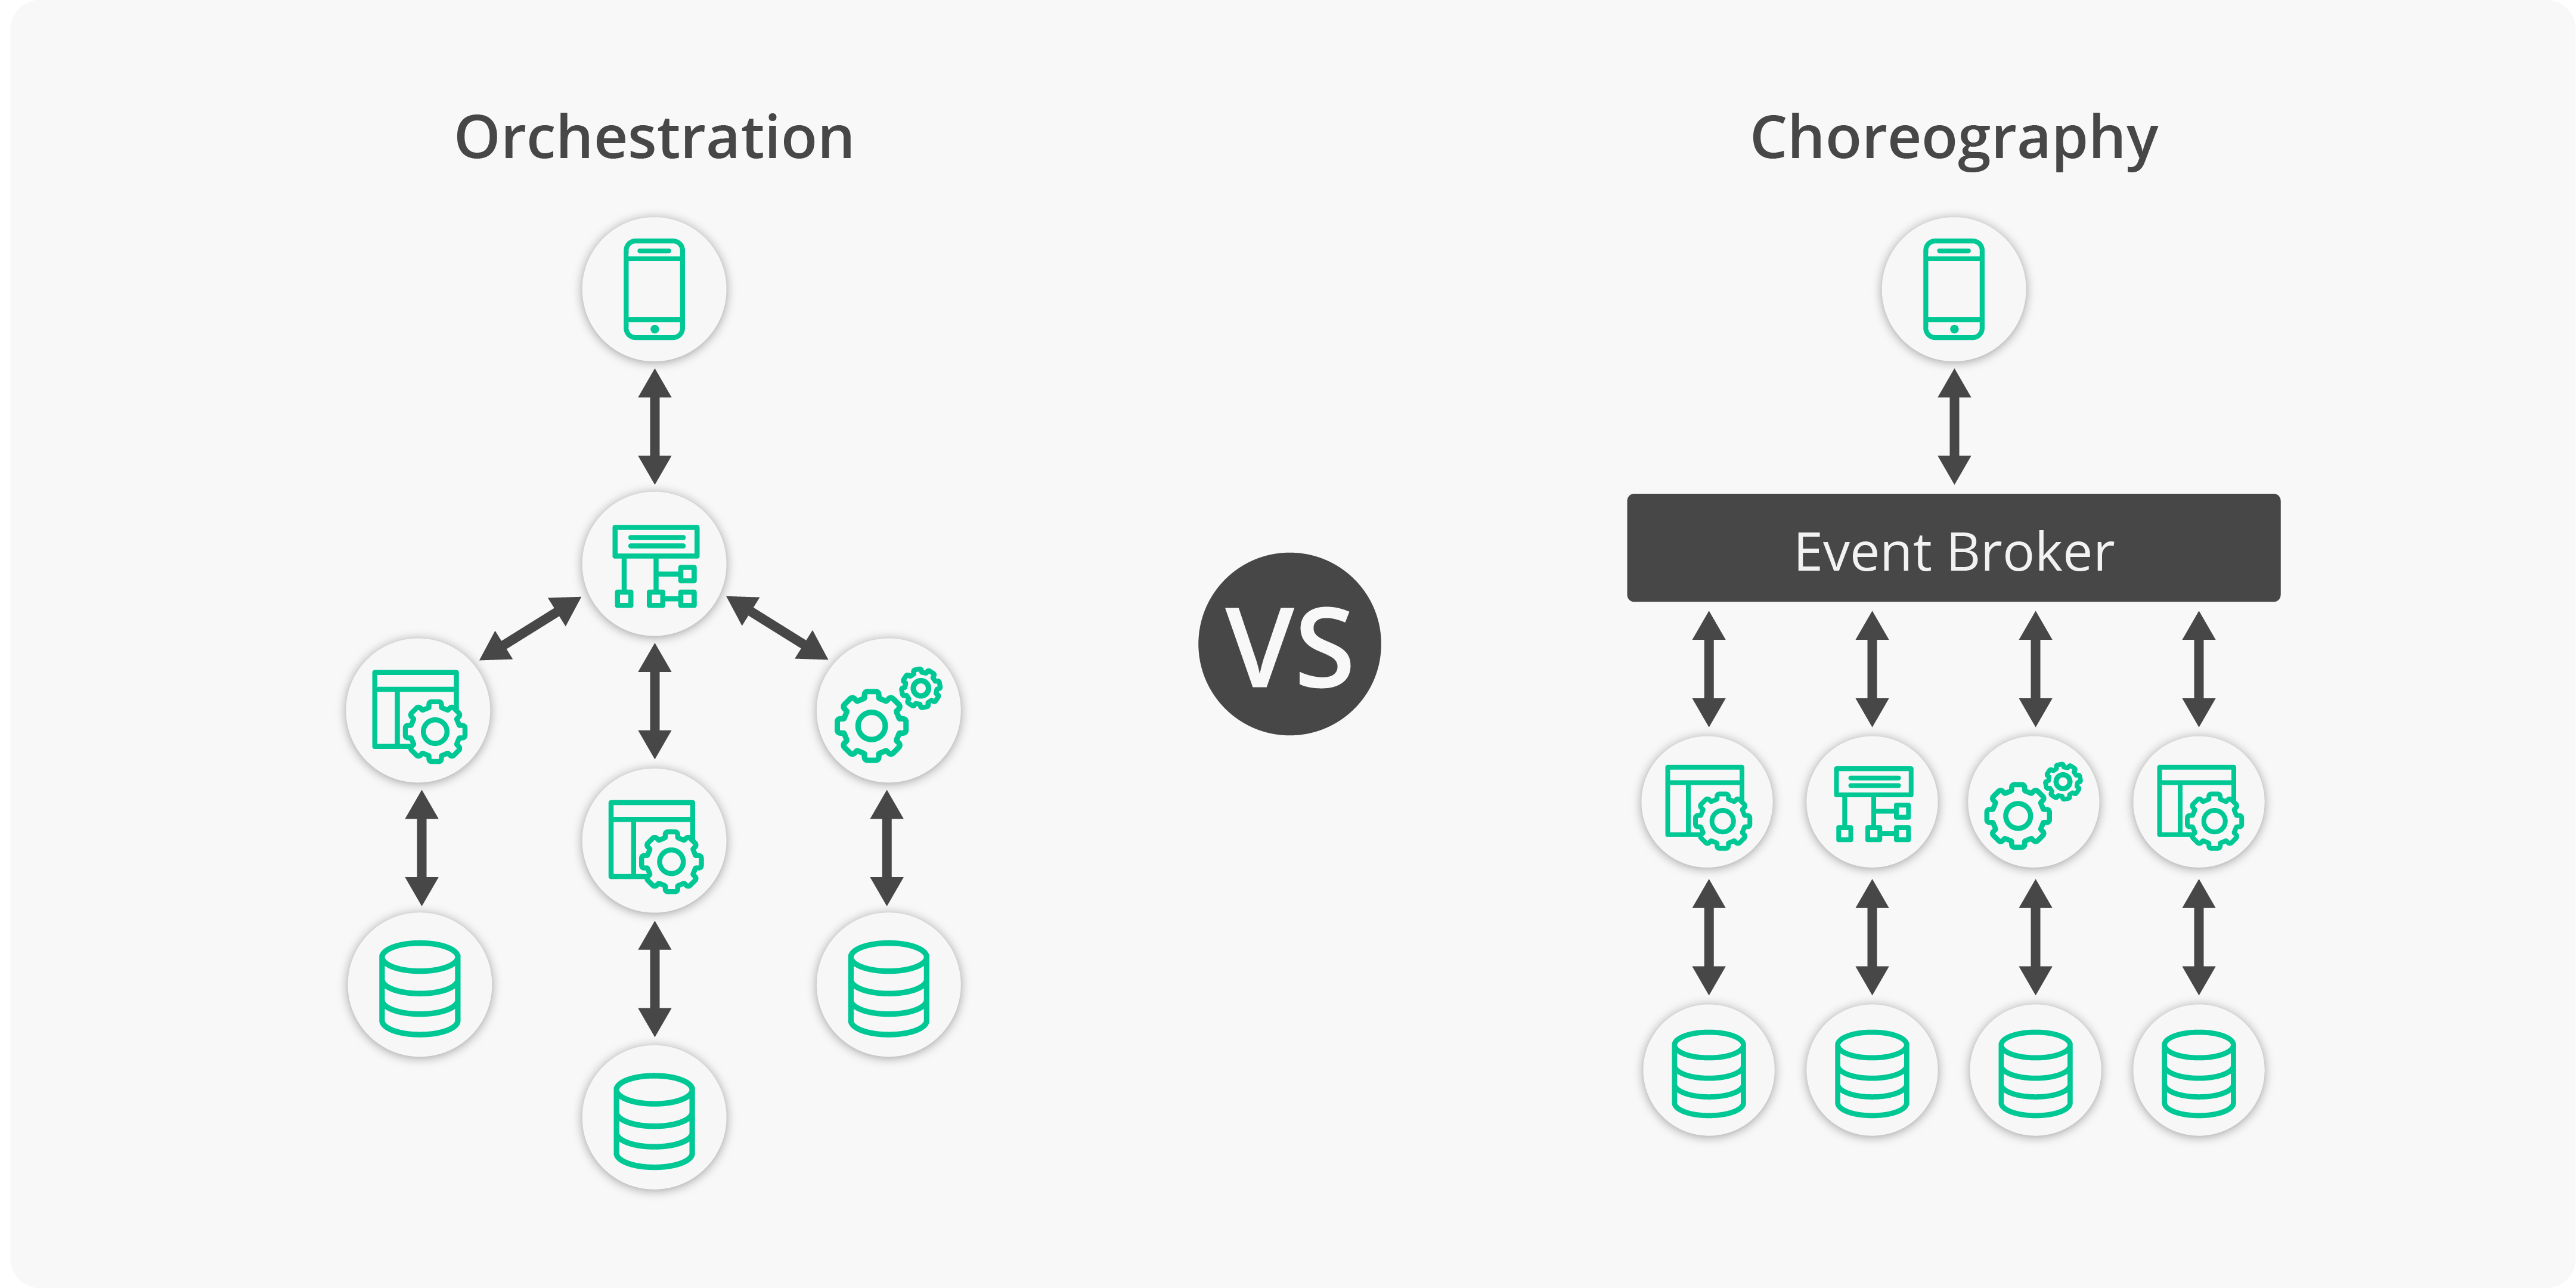
\includegraphics[width=1\textwidth]{images/Orchestration-VS-Choreography}
			 \caption{Orchestrare versus Coreografie}
			 \label{fig:orch_vs_coreografie}
			 \source {https://solace.com/blog/microservices-choreography-vs-orchestration/}
\end{center}
\end{figure}

\par Durable task framework, implementează o arhitectură de tip mediator central, si expune bazele pentru a putea crea propriul mediator pentru gestiunea unui workflow de lungă durată. Pentru a analiza implementarea conceptului de orchestrare bazată pe evenimente, vom analiza implementarea de DTF împreuna cu Sql Server Provider, pentru a face o transpunere a conceptelor teoretice în lumea DTF. În ~\ref{fig:sql-server-provider} se poate observa structura schemei ce susţine framework-ul atunci cand este rulat împreuna cu un SQL Server Provider. Acesta implementează conceptele teoretice intr-un nivel de stocare bazat pe SQL server. 
 
 \begin{figure}[h]
\begin{center}
        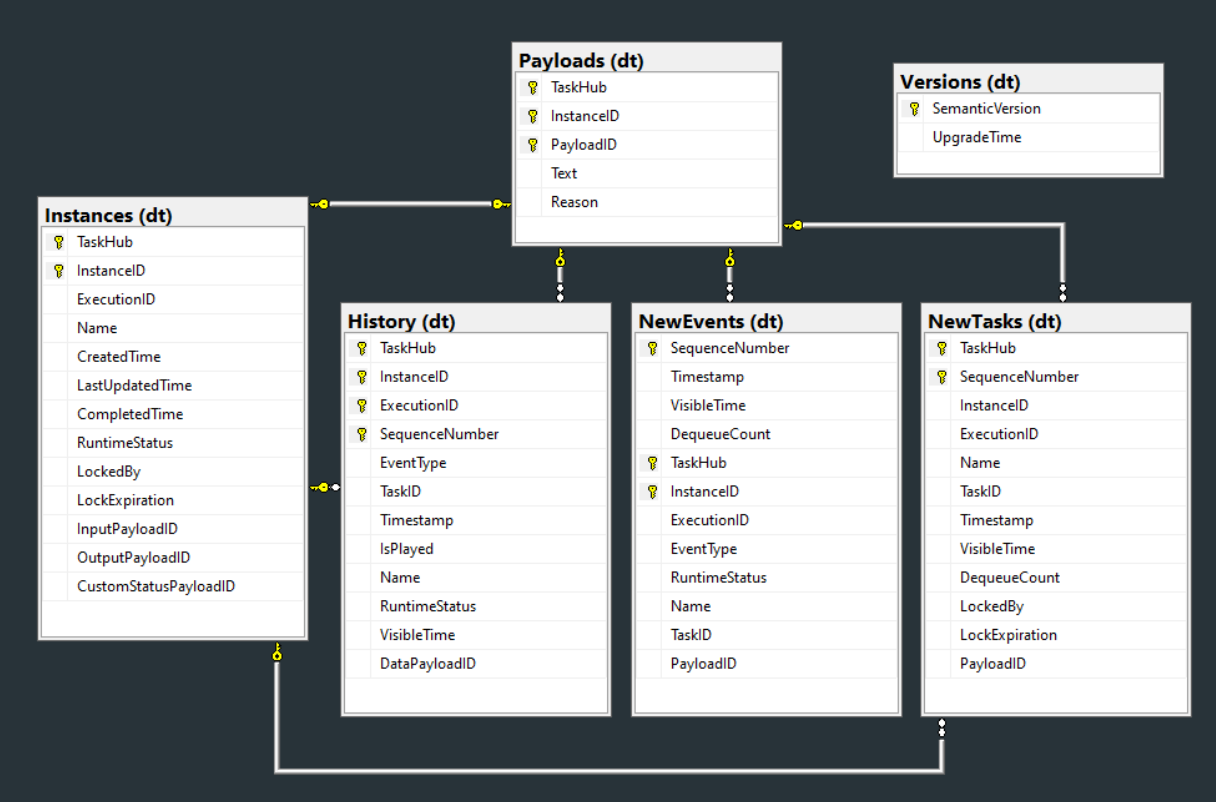
\includegraphics[width=1\textwidth]{images/sql-server-provider}
			 \caption{DTF Schema în DTF Sql Server provider}
			 \label{fig:sql-server-provider}
			 \source {https://microsoft.github.io/durabletask-mssql/}
\end{center}
\end{figure}

\par Există patru tipuri principale de componente de arhitectură în topologia mediatorului: 
\begin{itemize}
\item cozi de evenimente
\item mediatorul de evenimente
\item canale de evenimente
\item procesatoarele de evenimente. 
\end{itemize}
\par Fluxul de evenimente începe cu un client care trimite un eveniment la o coadă de evenimente, care este utilizată pentru a transporta evenimentul la mediatorul de evenimente. Mediatorul de evenimente primește evenimentul inițial și orchestrează acel eveniment prin trimiterea de evenimente asincrone suplimentare către canalele de evenimente pentru a executa fiecare pas al procesului. Procesatoarele de evenimente, care ascultă pe canalele de evenimente, primesc evenimentul de la mediatorul de evenimente și execută o logică de afaceri specifică pentru a procesa evenimentul.  Vom analiza fiecare componentă teoretică a procesului pentru a stabili parelela către structura din DTF, urmărind schema descride a ~\ref{fig:sql-server-provider}.
\par În cazul nostru, coada de eveniment este tabela `New Events` iar modalitatea prin care un eveniment ajunga în aceasta, este prin folosirea unui DTF Client pentru a inregistra un eveniment pentru o anumita orchestrare. 
\par Mediatorul de evenimente este `Orchestrarea` respectiv logica definită de dezvoltator pentru a gestiune workflow-ul. Această logica este rulată de fiecare dată când un eveniment este primit pentru un anume workflow. Deşi codul este rulat de mai multe ori, operaţiune denumita şi `Replay`, acţiunile care deja au mai fost executate odată nu sunt re-executate, ci rezultatele lor sunt direct încarcate direct din memorie, folosind istoricul orchestrării. Istoricul este salvat in tabela `History`.
\par Canalele de evenimente sunt diferitele Task-uri înregistrate în table NewTasks. Acestea sunt folosite de pentru a declanşă execuţia unor Activităţi, ce reprezintă frunzele arborelui de executie a unui workflow. Task-urile sunt înregistrate pe canalele de evenimente de catre mediatorul de evenimente, pentru a fi mai apoi procesate de procesatorul de evenimente. La finalul procesării unui task din canalul de evenimente, procesatorul de evenimente emite un nou eveniment pe coada de evenimente, pentru ca mediatorul să poate continua execuţia workflow-ului. 
\par Procesatoarele de evenimente sunt Workerii de DTF, si reprezintă logica din DTF Core care monitorizează în mod constant canalele de evenimente pentru a prelua eventualele noi Task-uri ce sunt disponibile pentru execuţie. Astfel, se obţine o arhitectură foarte decuplată în care inregistrarea de evenimente, gestionarea stării workflow-ului, execuţia propriu zisă a diverselor taskuri şi întoarcerea răspunsurilor inapoi către mediator sunt toate operaţiune decuplate, independente una de cealaltă.
\par Cel mai important aspect ce reiese din analiza implementării conceptelor de orchestrare bazată pe evenimente, este că datorită operaţiilor independente, eşecurile care pot apărea atunci cand această logica este executată într-un mediu distribuit nu vor afecta starea workflow-ului ca un întreg, fiindcă eşecul într-o parte a arhitecturii nu afectează alte părţi iar fiecare unitate este independent reîncercabilă. Astfel revenirea în urma unui eşec (eroare de reţea, deconectare completă fie a workerilor fie a client-ului) sunt gestionate într-un mod graţios, fără efecte secundare. 

\section{DTF în Durable Functions} 
\quad Conceptele prezentate în capitolul anterior, au fost reimpletate in DTF pentru a putea executa această tehnologie folosind soluţii native în cloud, şi pentru a expune o soluţie pentru care exista o mare nevoie în piaţă : Statefull Serverless functions. Astfel a fost dezvoltat un nou provider pentru DTF, bazat pe Azure Storage tables de această dată, pentru a expune aceeaşi functionalitate şi în cloud. 
\par Logica de bază a framework-ului a ramas aceeaşi în schimb implementarea celor 4 concepte de bază intr-o arhitectură bazată pe evenimente (cozi de evenimente,mediatorul de evenimente,canale de evenimente, procesatoarele de evenimente) este schimbată.
\par Această adaptare a dus la lansarea unei soluţii noi pe piaţă ce a creat un cu totul nou domeniu în lumea serverless. Funcţii ce sunt capabile ce gestioneze starea, si să ruleze o perioada foarte îndelungată de timp, dar pentru care se plăteşte doar timpul de execuţie propriu zis. Acest lucru vine cu beneficii foarte mari din punct de vedere al costurilor, deoarece într-un workflow ce conţine şi paşi manuali, cum ar fi aprobarea de către un operator a unei trazacţii, pe perioada în care se asteaptă acest eveniment, codul orchestrării nu se execută, deci practic nu există un cost asociat acestei operaţii. 
\par Pe lângă functionalităţile ce există în mod standard în toţi providerii de DTF, Durable Functions vine cu o caracteristică suplimentară numită Durable Entities. Durable Entities definesc operațiuni pentru citirea și actualizarea unor mici părți de stare, cunoscute sub numele de entități durabile. La fel ca funcțiile de orchestrator, funcțiile de entitate sunt funcții cu un tip de declanșator special, declanșatorul de entitate. Spre deosebire de funcțiile de orchestrator, funcțiile de entitate gestionează starea unei entități în mod explicit, mai degrabă decât să reprezinte implicit starea prin fluxul de control. Entitățile oferă un mijloc de extindere a aplicațiilor prin distribuirea lucrării în mai multe entități, fiecare cu o stare de dimensiuni modeste. Acest lucru practic oferă suport automat pentru gestiunea unei stări independente de cea a orchestrării, dar într-un mod distribuit si sigur, deoarece oferă garanţii de access serializat l-a aceasta. 
 \begin{figure}[h]
\begin{center}
        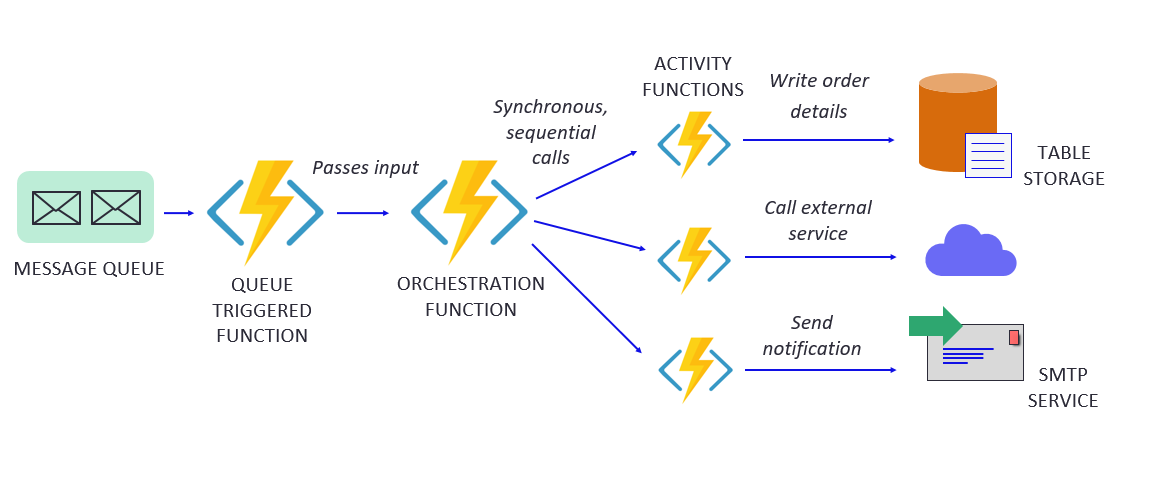
\includegraphics[width=1\textwidth]{images/durable-functions}
			 \caption{Exemplu arhitectură folosind Durable Functions}
			 \label{fig:durable-functions}
			 \source {https://thisiszone.medium.com}
\end{center}
\end{figure}
\par Aşa cum se poate observa şi în figura ~\ref{fig:durable-functions}, conceptele clasice de DTF sunt transpuse în functii individuale, de diferite tipuri. Astfel, o Orchestrare este reprezentata de un Orchestration Function, o activitate este reprezentată de un Activity Function, în timp ce starea globală a workflow-ului este stocată în tabele în Azure Storage. Obţinem astfel o arhitectură nativă în cloud, fară costuri de mentenanţă a infrastructurii şi de scalare, având ca beneficiu principal faptul că gestionarea stării într-un mediu distribuit nu mai este responsabilitatea explicită a dezvoltatorului, ci este rezolvată implicit de către providerul de soluţii cloud. 
\section {Greutăţi în gestionarea workflow-urilor de lunga durată - Versionarea Orchestrarilor }
\quad Pe langă beneficiile pe care le are o arhitectură bazată pe un mediator pentru gestiunea workflow-urilor, această centralizare are şi anumite limitări si dezavantaje. Printre aceastea, poate cel mai dificil lucru de gestionat este versionarea acestora.
\par Natura îndelungată a acestor workflow-uri face acestea sa aibă urmatoarele particularităţi: 
\begin{itemize}
\item Un workflow poate dura mai mult de un ciclu de dezvoltare (Mai multe versiuni ale aceluiaşi workflow pot exista până când o anumită instanţă a unei anume versiuni finalizează execuţia). 
\item Codul de orchestrare trebuie sa fie determinist deoarece acesta va fi executat de mai multe ori pe perioada de viaţă a unui workflow. 
\end{itemize}
\par Prima problema se rezumă la dificultatea de versionarea a unei orchestrări. Atunci cand aparea o versiunea nou a maşinii de stări gestionată de o anume orchestrare, cea veche nu poate fi direct înlocuită, deoarece încă există instanţe ale acelui tip de workflow care înca rulează. Astfel, versiunile noi de orchestrare trebuie mereu rulate în paralel cu cele vechi, până când toate instanţele ce rulează versiunea veche a workflow-urilor finalizează execuţia. În acel moment versiunea veche a orchestrării poate fi stearsă. 
\par Cea de doua problema este mai mult doar o limitare şi anume, din cauza logicii de replay multi pe perioada de viaţă a unei orchestrări, dezvoltatorul trebuie sa se asigura ca tot cod-ul din cadrul unei orchestrări, va returna acelaşi rezultat indiferent de momentul în care se rulează. Pe scurt, comportamentul unei orchestrări trebuie sa fie determinist si constant indiferent de timp. 
 \begin{figure}[h]
\begin{center}
        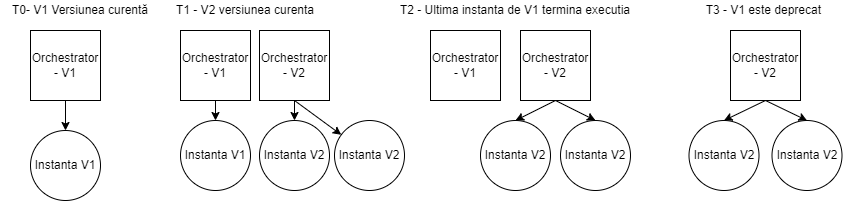
\includegraphics[width=1\textwidth]{images/dtf_versioning}
			 \caption{Ciclu de versionarea a codului de orchestrare}
			 \label{fig:dtf-versioning}
\end{center}
\end{figure}
\chapter{Workflow-uri de lungă durata - Analiză paralelă a arhitecturii}

\chapter {Rezultate şi Concluzii}

\section{Concluzii}

\bibliographystyle{abbrv}
\listoffigures
\listoftables
\bibliography{References}
\end{document}